%%%%%%%%%%%%%%%%%%%%%%%%%%%%%%%%%%%%%%%%%
% Beamer Presentation
% LaTeX Template
% Version 1.0 (10/11/12)
%
% This template has been downloaded from:
% http://www.LaTeXTemplates.com
%
% License:
% CC BY-NC-SA 3.0 (http://creativecommons.org/licenses/by-nc-sa/3.0/)
%
%%%%%%%%%%%%%%%%%%%%%%%%%%%%%%%%%%%%%%%%%

%----------------------------------------------------------------------------------------
%	PACKAGES AND THEMES
%----------------------------------------------------------------------------------------

\documentclass{beamer}

\mode<presentation> {

% The Beamer class comes with a number of default slide themes
% which change the colors and layouts of slides. Below this is a list
% of all the themes, uncomment each in turn to see what they look like.

%\usetheme{default}
%\usetheme{AnnArbor}
%\usetheme{Antibes}
%\usetheme{Bergen}
%\usetheme{Berkeley}
%\usetheme{Berlin}
%\usetheme{Boadilla}
%\usetheme{CambridgeUS}
%\usetheme{Copenhagen}
%\usetheme{Darmstadt}
%\usetheme{Dresden}
%\usetheme{Frankfurt}
%\usetheme{Goettingen}
%\usetheme{Hannover}
%\usetheme{Ilmenau}
%\usetheme{JuanLesPins}
%\usetheme{Luebeck}
\usetheme{Madrid}
%\usetheme{Malmoe}
%\usetheme{Marburg}
%\usetheme{Montpellier}
%\usetheme{PaloAlto}
%\usetheme{Pittsburgh}
%\usetheme{Rochester}
%\usetheme{Singapore}
%\usetheme{Szeged}
%\usetheme{Warsaw}

% As well as themes, the Beamer class has a number of color themes
% for any slide theme. Uncomment each of these in turn to see how it
% changes the colors of your current slide theme.

%\usecolortheme{albatross}
%\usecolortheme{beaver}
%\usecolortheme{beetle}
%\usecolortheme{crane}
%\usecolortheme{dolphin}
%\usecolortheme{dove}
%\usecolortheme{fly}
%\usecolortheme{lily}
%\usecolortheme{orchid}
%\usecolortheme{rose}
%\usecolortheme{seagull}
%\usecolortheme{seahorse}
%\usecolortheme{whale}
%\usecolortheme{wolverine}

%\setbeamertemplate{footline} % To remove the footer line in all slides uncomment this line
%\setbeamertemplate{footline}[page number] % To replace the footer line in all slides with a simple slide count uncomment this line

%\setbeamertemplate{navigation symbols}{} % To remove the navigation symbols from the bottom of all slides uncomment this line
}

\usepackage{graphicx} % Allows including images
\usepackage{booktabs} % Allows the use of \toprule, \midrule and \bottomrule in tables

%----------------------------------------------------------------------------------------
%	TITLE PAGE
%----------------------------------------------------------------------------------------

\title[Model Compexity]{Controlling Model Complexity} % The short title appears at the bottom of every slide, the full title is only on the title page

\author{Dale Smith} % Your name
\institute[Consulting Data Scientist] % Your institution as it will appear on the bottom of every slide, may be shorthand to save space
{
Atlanta, GA \\ % Your institution for the title page
%\medskip
%\textit{dale.smith.phd@gatech.edu} % Your email address
}
\date{\today} % Date, can be changed to a custom date

\begin{document}

\begin{frame}
\titlepage % Print the title page as the first slide
\end{frame}

\begin{frame}
\frametitle{Overview} % Table of contents slide, comment this block out to remove it
\tableofcontents % Throughout your presentation, if you choose to use \section{} and \subsection{} commands, these will automatically be printed on this slide as an overview of your presentation
\end{frame}

%----------------------------------------------------------------------------------------
%	PRESENTATION SLIDES
%----------------------------------------------------------------------------------------

%------------------------------------------------
\section{Introduction}
\subsection{BioTech - Opportunities of Scale}
\subsection{BioTech Firms in Atlanta}
\section{Algorithms and Models}
\subsection{Models are Algorithms Fit to Data}
\subsection{Model Complexity}
\subsection{Example of Model Complexity and Overfitting}
\section{Regularization}
\subsection{Control the Complexity}
\subsection{Early Stopping}
\subsection{Control Model Complexity}
\subsection{Introducing Sparsity}
\subsection{ElasticNet}

\begin{frame}
\frametitle{BioTech - Opportunities of Scale}
\begin{itemize}
\item Cost of sequencing a single person's genome - \$3 bln 1989 -- 2001 to under \$1k today
\item Twelve years to sequence one versus multiple person's genome in under a week
\item Sequence DNA from skin cancer tumor versus sequence DNA from skin cells
\item Individualized treatments
\item Labiotech.eu: "The Robots are Coming: Is AI the Future of Biotech?"
\end{itemize}
\end{frame}

\begin{frame}
\frametitle{Biotech Firms in Atlanta}


\includegraphics{gra}

\end{frame}

%------------------------------------------------

\begin{frame}
\frametitle{Models are Algorithms Fit to Data}
\begin{equation}
y = f(x)
\end{equation}
\begin{itemize}
\item $x$ -- called features or independent variables
\item $y$ -- response variable, predicted quantity, dependent variable
dataset
\end{itemize}
\end{frame}

\begin{frame}
\frametitle{Models are Algorithms Fit to Data}
\begin{equation}
y = f(x)
\end{equation}
\begin{itemize}
\item Use future $x$ data in the model to generate a $y$
\item If $y$ is a set of classes, the problem is called a classification problem
\item Otherwise, $y$ is a continuous variable and it's a regression problem
\item Separate dataset into training, (validation), test sets, reflecting the characteristics of the undivided dataset \end{itemize}
\end{frame}

\begin{frame}
\frametitle{Model Complexity}
\begin{equation}
y = f(x)
\end{equation}
\begin{itemize}
\item Parsimonious models
\item Computation time for fit - determine model parameters from the data
\item Choosing hyperparameters - free parameters supplied by the user
\end{itemize}
\end{frame}

\begin{frame}
\frametitle{Example of Model Complexity and Overfitting}
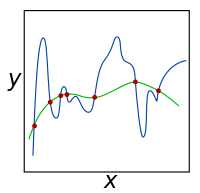
\includegraphics{overfit}
\begin{itemize}
\item Overfitting: low training error, high test error - lack of generalization
\end{itemize}
\end{frame}

\begin{frame}
\frametitle{Regularization - Control the Complexity}
\begin{itemize}
\item Fitting or training a model is an ill-posed problem
\item Every model or algorithm requires a fit process to determine unknown parameters
\item The fit process is eventually recast as an optimization problem
\item Simpler model
\item Sparse model
\item Basic principle - cost function + a complexity penalty
\end{itemize}
\end{frame}

\begin{frame}
\frametitle{Regularization - Early Stopping}
\begin{itemize}
\item Regularization in time
\item When the model performance doesn't improve on the validation set, stop
\item Evaluate once more on test set to estimate generalization error
\item Often used with neural networks and tree-based algorithms
\end{itemize}
\end{frame}

\begin{frame}
\frametitle{Regularization - Control Model Complexity}
\begin{align}
y &= f(x) \\
C(x, y) &= \min_f \sum_{i=1}^{n} \left| f(x_i) - y_i \right|^2 + \lambda \| f \|_2^2
\end{align}
\begin{itemize}
\item All parameters are driven to zero (but not all are non--zero)
\item The underlying optimization problem can be solved with minimizers which require first and second derivatives
\item These methods are more accurate and faster than minimizers which do not use gradient information
\item There may be explicit matrix solutions
\end{itemize}
\end{frame}

\begin{frame}
\frametitle{Regularization - Introducing Sparsity}
\begin{itemize}
\item We want the model to have many data-dependent or algorithm parameters zero
\item Sometimes use the number of non--zero parameters
\item Use the sum of the absolute value - $| \beta_1 | + | \beta_2 | + \cdots + | \beta_m |$
\item This drives parameters to zero, except for a few
\item Correlated features have a few representatives included, the others are not included
\end{itemize}
\end{frame}

\begin{frame}
\frametitle{Regularization - ElasticNet}
\begin{align}
y &= f(x) \\
C(x, y) &= \min_f \sum_{i=1}^{n} \left| f(x_i) - y_i \right|^2 + \lambda \left( \alpha \| f \|_2^2 + (1 - \alpha) \sum \left| \beta_i \right| \right)
\end{align}
\begin{itemize}
\item Use the measures $\|. \|^2$ and $|.|$ together
\item $\lambda$ and $\alpha$ are hyperparameters that must be chosen via \textit{cross-validation} or some other method
\item Correlated features are assigned equal weights
\end{itemize}
\end{frame}

%------------------------------------------------

\begin{frame}
\frametitle{The End}
\Huge{\centerline{The End - Thank You for Listening!}}
\end{frame}

%----------------------------------------------------------------------------------------

\end{document} 